%chapter-Apportionment.tex

%<*CHAPTERHEADER>

\declareproblemlettering{D}
\pagestyle{fancy}
\cleartooddpage

\chapter{Apportionment and Division}\label{ch:division}

\section{Apportionment} 
\index{apportionment}
Another mathematical challenge in most Democratic systems is that of Apportionment.  Essentially the problem is one of representation.  Seats in the House of Representatives are given to the states based on population.  There are 435 seats for 2323.1 million people.  That works out to $323100000/435 = 742758.6207$ or about $742,759$ people per seat in the House.  However, even though North Dakota, Vermont, and Wyoming all have smaller populations than that they are guaranteed a seat in the House.  Also, if you look at the other states, it is very rare that their population is exactly an even multiple of $742,759$.  This section is all about how to fairly appoint seats in a house of representatives, as well as a variety of other tasks that turn out to be essentially the same thing.

\begin{enumerate}
		\item The Republic of Awoi is a small country consisting of four states North-West (population 69,000), South-West 	(population 267,000), South-East (population 133,000) and North-East (population 331,000).  Suppose that there are 160 seats in the Awoi Congress to be apportioned among the four states based on their representative populations.
		\begin{enumerate}
			\item On average, how many people per congress seat should there be?\ifsolns \par 5000 \else
	\fillwithlines{\stretch{1}}
\fi
	

			\item How would you give out the 160 seats to the four states and why?
			\large
			
			\ifsolns
			\begin{tabular}{c|c|c|c|c} \hline
				& NW & SW & SE & NE \\\hline
				Seats &14&53&27&66 \\\hline
			\end{tabular}
	\end{enumerate}\vfill
	\else
			\begin{tabular}{c|c|c|c|c} \hline
				& NW & SW & SE & NE \\\hline
				Seats &&&& \\\hline
			\end{tabular}
	\end{enumerate} 
	\fillwithlines{\stretch{1}}\fi
\normalsize
\clearpage
	
	\item Notes on Apportionment
	\vfill
	 \boxedblank[2in]{\textbf{Standard Divisor (SD):}\solution{The whole population divided by the number of seats}\fillwithlines{\stretch{1}}} \index{divisor!standard}
	 
  \boxedblank[2in]{\textbf{Standard quotas ($q_1,q_2,\dots q_N$):}\solution{Population of each state divided by the standard divisor.}\fillwithlines{\stretch{1}}} \index{quota!standard}
	  
   \boxedblank[2in]{\textbf{Upper and lower quotas:}\solution{The upper quota is the standard quota rounded up and the lower quota is the standard quota rounded down.  A fair apportionment will lead to all states having either their upper or lower quota.}\fillwithlines{\stretch{1}}} \index{quota!upper} \index{quota!lower}
	   \vfill

	\clearpage
\subsection{Hamilton's Method} \index{apportionment method!Hamilton}
	\item 	   \boxedblank[2in]{\textbf{Hamilton's Method:}\solution{Assign all states their lower quota.  Then, to assign the extra seats, look at the state with the largest decimal part in its standard quota and assign it the upper quota.  Continue until all extra seats are assigned.}}
	\vfill
	\item Consider the Republic of Awoi:
	\begin{enumerate}
			\item Find the standard divisor. \solution{5,000}
			\fillwithlines{\stretch{1}}
			%\large
		{\renewcommand{\arraystretch}{2}
		
\begin{tabular}{c|c|c|c|c|c} \hline
	 & Population  & Standard quota  & LQ  & UQ  & App \\\hline
\ifsolns NW  & 69,000 & 13.8 & 13 & 14 & 14\\\hline
 SW  & 267,000 & 53.4 & 53 & 54 & 53\\\hline
 SE  & 133,000 & 26.6 & 26 & 27 & 27\\\hline
 NE  & 331,000 & 66.2 & 66 & 67 & 66\\\hline
	\else
 NW  & 69,000 &  &  &  & \\\hline
 SW  & 267,000 &  &  &  & \\\hline
 SE  & 133,000 &  &  &  & \\\hline
 NE & 331,000 &  &   &   & \\\hline
	\fi		\end{tabular}
	}
		\normalsize
		
		In the table above:
		\item Find each state's standard quota.
		\item Find each state's lower and upper quota.
		\item Find the apportionment as described by Hamilton's Method.
	\end{enumerate} \vfill
	
	\clearpage
	\item The Republic of Bananarama is  a small country consisting of five states ($A, B, C, D,$ and $E$).  The total population of Bananarama is 23.8 million.  According to the Bananarama constitution, the seats in the legislature are apportioned to the states according to their populations.  The following table shows each state's standard quota:
	
	\begin{center}
	\begin{tabular}{lcccccc}
State & $A$ & $B$ & $C$ & $D$ & $E$ \\\hline
Standard quota &40.50 & 29.70 & 23.65 & 14.60 & 10.55 \\\hline
\end{tabular}
\end{center}
	
	In the Table below:
	\begin{enumerate}
	
	
	\item Find the number of seats in the Bananarama legislature.
	\item Find the Standard Divisor.
	\item Find the population of each state.

	\begin{center}
	\begin{tabular}{l|c|c|c|c|c} \hline
State	&	Pop. &Q. &	LQ&  Additional Seats	 	&  	 	Apportionment \\\hline
\ifsolns	$A$ &8.1&40.5&40&&40\\\hline
	$B$ &5.94&29.7&29&1&30\\\hline
	$C$ &4.73&23.65&23&1&24\\\hline
	$D$ &2.92&14.6&14&1&15\\\hline
	$E$ &2.11&10.55&10&&10\\\hline
	Totals &23.8&200,000&119&&116\\\hline
	\else
	$A$ &&&&&\\\hline
	$B$ &&&&&\\\hline
	$C$ &&&&&\\\hline
	$D$ &&&&&\\\hline
	$E$ &&&&&\\\hline
	Totals &&&&&\\\hline \fi
	\end{tabular}
	
	\end{center}

	\item Find each state's standard lower quota.
	\item Find the apportionment as described by Hamilton's method.
\end{enumerate}


\end{enumerate}
%\clearpage
\clearpage
{\large Worksheet for calculating Hamilton's Method:}

\begin{enumerate}
	\item What is the total population? \hrulefill
	\item How many seats are you apportioning\footnote{If you aren't given this number, it is the total of the Standard Quotas}?  \hrulefill
	\item Calculate the Standard Divisor (divide your population by the number of seats):  \hrulefill
	\item Calculate all the Standard Quotas (Q.) (divide the population of each state by your Standard Divisor).  The total of your standard quotas should be the same as the number of seats.  If that is not the case, you have rounded off too much.:
	
	\begin{center}
			\begin{tabular}{l|c|c|c|p{36pt}|p{36pt}} \hline
	State	&	Pop. &Q. &	LQ&  Addi\-tional Seats	 	&  	 	Appor\-tionment \\\hline
\raisebox{0pt}[72pt][72pt]{\makebox[36pt]{}}&\makebox[36pt]{}&\makebox[36pt]{}&\makebox[36pt]{}&\makebox[36pt]{}&\makebox[36pt]{}\\ \hline
Totals &&&&&\\
		\end{tabular}
	\end{center}
	\item Write down all the Lower Quotas (LQ) by cutting off the decimal places.  The total of your lower quotas should be less than the number of seats.  The difference between the two is the additional seats you get to give out.
	\item Give out your additional seats by giving one seat to each state ranked by the stuff to the right of the decimal point on the standard quotas.
\end{enumerate} 
\clearpage
%%%%%%%%%%%%%%%%%%%%%%%%%%%%%%%%%%%%%%%%%%%%%%%%%%%%%%%%%%%%%%%%%%%%%%%%%%%%%%%%%%%%%%%%%%%%%%%%%%
\HOMEWORK

Show all your work.

\begin{Denumerate}

	\item Waterloo General Hospital has a nursing staff of 175 nurses working in four shifts: $A$ (7:00 AM to 1:00 PM), $B$ (1:00 PM to 7:00 PM), $C$ (7:00 PM to 1:00 AM), $D$ (1:00 AM to 7:00 AM).  The number of nurses apportioned to each shift is based on the average number of patients treated in that shift, given in the following table:

	\begin{center}
	%\large

		\begin{tabular}{lr|c|c|c|c}
	\hline
	Shift &	Patients & Standard Quota & Lower Quota & Additional & Apportionment \\\hline
\ifsolns$ A $ & 871 & 56.4537 & 56 &  & 56\\\hline 
$ B $ & 1029 & 66.69444 & 66 & 1 & 67\\\hline 
$ C$ & 610 & 39.53704 & 39 & 1 & 40\\\hline 
$D $ & 190 & 12.31481 & 12 &  & 12\\\hline 
Total  & 2700 & 175 & 173 &  & 175\\\hline \else
	 $A$ &	871 &&&&\\\hline
	 $B$ &	1029&&&&\\\hline
	 $C$&	610&&&&\\\hline
	$D$ &	190&&&&\\\hline
	Total && 175 &&&\\\hline \fi
	\end{tabular}
	
	\normalsize
	\end{center}	
	
	\begin{enumerate}
		\item Find the standard divisor. \solution*{15.42857143}
		\item Explain what the standard divisor represents in this problem. \solution*{One nurse will be assigned for each 15.4 patients.}\vspace{2in}
		\item Find the standard quotas.
		\item Using Hamilton's Method, assign extra seats to the lower quotas, one at a time, until you have apportioned all your nurses.
		\item Find the apportionment based on Hamilton's method. 
		\solution*{\begin{tabular}{cc}
		$ A $ & 56\\
$ B $ & 67\\
$ C$ & 40\\
$D $ & 12\\
		\end{tabular}}\vfill
	\end{enumerate}

\hwnewpage
	\item Southern Iowa University is made up of five different schools: Agriculture, Business, Education, Humanities, and STEM ($A$, $B$, $E$, $H$, and $S$ for short).  The 250 faculty positions at SIU are apportioned to the various schools based on the schools' representative enrollments.  The following table shows each school's enrollments:

	\begin{center}
	%\large
		\begin{tabular}{lr|c|c|c|c}
	\hline School &	Enrollment & S Q & L Q & Additional & Apportionment \\\hline \ifsolns
	$A$ & 3292 & 32.92 & 32 & 1 & 33\\\hline
$B$ & 1524 & 15.24 & 15 &  & 15\\\hline
$E$ & 4162 & 41.62 & 41 & 1 & 42\\\hline
$H$ & 2132 & 21.32 & 21 &  & 21\\\hline
$S$  & 13890 & 138.9 & 138 & 1 & 139\\\hline
Total  & 25,000 & 250 & 247 & 3 & 250\\\hline
\else
	$A$&	3292&&&&\\\hline
	$B$	&1524&&&&\\\hline
	$E$	&4162&&&&\\\hline
	$H$	&2132&&&&\\\hline
	$S$ &	 13890 &&&&\\\hline
	Total & 25,000 & 250 &&&\\\hline \fi
	\end{tabular}
	\normalsize
	\end{center}


	\begin{enumerate}
		\item
		 Find the standard divisor. \solution{ 100}
		\item Explain what the standard divisor represents in this problem. \solution{Each faculty member is responsible for 100 students, or the student to faculty ratio is 100.}\vspace{2in}
		\item Find the standard quotas.
		\item Find the apportionment based on Hamilton's method.
	\end{enumerate}

\end{Denumerate} \ENDHOMEWORK
%%%%%%%%%%%%%%%%%%%%%%%%%%%%%%%%%%%%%%%%%%%%%%%%%%%%%%%%%%%%%%%%%%%%%%%%%%%%%%%%%%%%%%%%%%%%%%%%%%%%%%

\clearpage
\subsection{Paradoxes} \index{paradoxes!Apportionment}
\begin{enumerate}
	\item The small country of Amabala consists of three states: Eno, Owt, and Eerht.  With a total population of 20,000 and 200 seats in the House of Representatives the apportionment of the 200 seats under Hamilton's method is shown below:

	\begin{center}
		\begin{tabular}{lrrrrr} \hline
	State & Population & Quota & Lower quota & Additional & Apportionment \\\hline
	Eno & 940 & 9.4 & 9 & 1 & 10 \\\hline
	Owt & 9030 & 90.3 & 90 & 0 & 90 \\\hline
	Eerht & 10,030 & 100.3 & 100 & 0 & 100 \\\hline\hline
	Total & 20,000 & 200.0 & 199 & 1 & 200 \\\hline
	\end{tabular}
	\end{center}
	What was the Standard Divisor that was used to apportion Amabala's seats? \ifsolns 100 \fi\hrulefill
	
	Now, imagine that the number of seats is suddenly \textbf{increased to 201}, but \textbf{nothing else changes}.  Since there is one more seat to give out, the apportionment has to be recomputed.
	\begin{enumerate}
		\item What is the new Standard Divisor?  It has to change because the number of seats has changed.  \ifsolns 99.50 \fi \hrulefill
	
	\begin{center}
	\large
		\begin{tabular}{l|r|r|r|r|r} \hline
	State & Population & SQ & LQ & Additional & Apportionment \\\hline
	\ifsolns
	Eno  & 940 & 9.447 & 9 &  & 9\\\hline 
Owt  & 9030 & 90.7515 & 90 & 1 & 91\\\hline 
Eerht  & 10,030 & 100.8015 & 100 & 1 & 101 \\\hline \hline
Total  & 20,000 & 201 & 199 & 2 & 201 \\\hline 
\else
	Eno & 940 &  &  &  &  \\\hline
	Owt & 9030 &  &  &  &  \\\hline
	Eerht & 10,030 &  &  &  &  \\\hline \hline
	Total & 20,000 & 201 &  &  &  \\\hline \fi
	\end{tabular}
	\normalsize
	\end{center}
	
	
		\item Which state received an extra seat?\hrulefill
		%\fillwithlines{\stretch{1}}
		\item Which state lost a seat?\hrulefill
		%\fillwithlines{\stretch{1}}
		\item What do you find odd about this situation? \hrulefill
		\fillwithlines{\stretch{1}}
	\end{enumerate}

	\item \boxedblank[2in]{\textbf{Alabama Paradox:}\fillwithlines{\stretch{1}}} \index{paradox!Alabama}
\clearpage
	\item Consider the following apportionment made using Hamilton's method.  Populations are given in millions:
	
	\begin{center}
		\begin{tabular}{lrrrrr} \hline
	State & Population & Quota & Lower quota & Additional & Apportionment \\\hline
	Alpha & 150 & $8.\overline{3}$ & 8 & 0 & 8 \\\hline
	Beta & 78 & $4.\overline{3}$ & 4 & 0 & 4 \\\hline
	Gamma & 173 & $9.6\overline{1}$ & 9 & 1 & 10 \\\hline
	Delta & 204 & $11.3\overline{3}$ & 11 &0 & 11 \\\hline
	Epsilon & 295 & $16.3\overline{8}$ & 16 & 1 & 17 \\\hline\hline
	
	Total & 900 & 50 & 48 & 2 & 50 \\\hline
	\end{tabular}
	\end{center}
	
	Ten years later a new census was taken which showed only a few changes in state populations -- an 8 million increase in the population of Gamma and a 1 million increase in the population of Epsilon.  \emph{The populations of the other states remained unchanged.}  Use Hamilton's method to calculate the new apportionment.
	\begin{enumerate}
		\item What is the new Standard Divisor?  It has to change because your total population has changed. \ifsolns 18.18 people/seat \fi \hrulefill
	
	\begin{center}
\ifsolns \else	\large\fi
		\begin{tabular}{l|r|r|r|r|r} \hline
	State & Population & Q & LQ & Additional & Apportionment \\\hline
	\ifsolns
	Alpha  & 150 & 8.250825083 & 8 &  & 8\\\hline 
Beta  & 78 & 4.290429043 & 4 & 1 & 5\\\hline 
Gamma  & 181 & 9.9559956 & 9 & 1 & 10\\\hline 
Delta  & 204 & 11.22112211 & 11 &  & 11\\\hline 
Epsilon  & 296 & 16.28162816 & 16 &  & 16\\\hline \hline
Total  & 909 & 50 & 48 & 2 & 50 \\\hline 
\else
	Alpha & 150 &&&& \\\hline
	Beta & 78 &&&& \\\hline
	Gamma & 181 &&&& \\\hline
	Delta & 204 &&&& \\\hline
	Epsilon & 296 &&&& \\\hline \hline
	Total & \textbf{909} & 50.00 &  &  & 50 \\\hline\fi
	\end{tabular}
	\normalsize
	\end{center}

		\item Which state received an extra seat?\hrulefill
		%\fillwithlines{\stretch{1}}
		\item Which state lost a seat?\hrulefill
		%\fillwithlines{\stretch{1}}
		\item What do you find odd about this situation?\hrulefill\fillwithlines{\stretch{1}}
	\end{enumerate}
	\item \boxedblank[2in]{\textbf{Population Paradox:} } \index{paradox!population}

\clearpage

	\item The W-CF Garbage Company has a contract to provide garbage collection and recycling services to the two towns of Waterloo (with 89,550 homes) and Cedar Falls (with 10,450 homes).  The company runs 100 little garbage trucks, which are apportioned under Hamilton's method according to the number of homes in the district.  A quick calculation shows that the standard divisor is $SD=1000$ homes, a nice, round number which makes the rest of the calculations easy.  
	
		\begin{center}
		\begin{tabular}{l|r|r|r} \hline
	State & Population & Q  & Apportionment \\\hline
	Waterloo & 89,550 &89.55&90 \\\hline
	Cedar Falls & 10,450 &10.45&10 \\\hline\hline
	Total & 100,000 & 100.00 & 100 \\\hline
	\end{tabular}
	\end{center}

	Now, the W-CF Garbage Company is bidding to expand its territory by adding the town of Evansdale (5250 homes) to its service area.  In the bid, the company promises to buy five additional garbage trucks for the Evansdale run so that its service to the other two towns is not affected.  Calculate the new apportionment.
		\begin{enumerate}
		\item What is your new Standard Divisor?  It will probably change because you have changed both your total population and the number of seats. \ifsolns 1002.38 \fi \hrulefill
	\large
		\begin{center}
		\begin{tabular}{l|r|r|r} \hline
	State & Population & Q  & Apportionment \\\hline \ifsolns
	Waterloo  & 89550 & 89.33729216   & 89\\\hline
Cedar Falls  & 10450 & 10.42517815 & 11\\\hline
Evansdale  & 5250 & 5.237529691  & 5\\\hline\hline
\else
	Waterloo & 89,550 && \\\hline
	Cedar Falls & 10,450 && \\\hline
	Evansdale & 5250 && \\\hline\hline\fi
	Total & 105,250 & 105.00 & \\\hline
	\end{tabular}
	\normalsize
	\end{center}
	
		\item Which city received an extra garbage truck?\hrulefill
		%\fillwithlines{\stretch{1}}
		\item Which state lost a garbage truck?\hrulefill
		%\fillwithlines{\stretch{1}}
		\item What do you find odd about this situation?\hrulefill\fillwithlines{\stretch{1}}
	\end{enumerate}
	\item \boxedblank[2in]{\textbf{New-States Paradox} \index{paradox!new-states}}
\end{enumerate}
%\end{enumerate}

\clearpage
%%%%%%%%%%%%%%%%%%%%%%%%%%%%%%%%%%%%%%%%%%%%%%%%%%%%%%%%%%%%%%%%%%%%%%%%%%%%%%%%%%%%%%%%%%%%%%%%%%%%
\HOMEWORK
The following problems are based on the following story:  Your professor found a stash of fun, math toys in her office.  She decides to apportion the toys among her three first-year advisees according to the number of minutes each student spent doing homework during the week.
\begin{Denumerate}
\item \studentrand \begin{enumerate}
	\item Suppose that there were 11 toys in the office.  Given that \randstudent[1]\ did homework for a total of 54 minutes, \randstudent[2]\ did homework for a total of 243 minutes and \randstudent[3]\ did homework for a total of 703 minutes, apportion the 11 toys among the students using Hamilton's method.
	\solution{\randstudent[1]\ - 0\\
\randstudent[2]\ - 3\\
\randstudent[3]\ - 8}
	\vfill \label{AppPar1}
	\item Suppose that before the professor hands out the toys, each student decides to spend a ``little'' extra time on homework.  \randstudent[1]\ puts in an extra 2 minutes (for a total of 56 minutes), \randstudent[2]\ put in an extra 12 minutes (for a total of 255 minutes), and \randstudent[3]\ an extra 86 minutes (for a total of 789 minutes).  Using these new totals, apportion the 11 toys among the students using Hamilton's method.
	\solution{\randstudent[1]\ - 1\\
\randstudent[2]\ - 2\\
\randstudent[3]\ - 8
}
	\vfill
	\item These results illustrate one of the paradoxes of Hamilton's method.  Which one?  Explain? \solution*{This is the Population Paradox.  Be sure to explain how you know.}
	\vfill
	\end{enumerate}
	
	\hwnewpage
\item \begin{enumerate}
	\item Suppose there were only 10 toys in the office Given that \randstudent[1]\ did homework for a total of 54 minutes, \randstudent[2]\ did homework for a total of 243 minutes and \randstudent[3]\ did homework for a total of 703 minutes, apportion the 10 toys among the students using Hamilton's method. \solution{Ben - 1, 
Paul - 2, 
Ryan - 7}

	\vfill
	\item Suppose that, just before she hands out the toys, the professor finds one additional math toy.  Using the same total minutes as above, apportion now the 11 math toys among the students using Hamilton's method.  [This is a repeat of Homework~\ref{AppPar1}.] \solution{Ben - 0, 
Paul - 3, 
Ryan - 8}
	\vfill
	\item These results illustrate one of the paradoxes of Hamilton's method.  Which one?  Explain? \solution{Alabama Paradox}
	\vfill
	\end{enumerate}
	
	\hwnewpage
\item \begin{enumerate}
	\item Suppose that there were 11 toys in the office.  Given that \randstudent[1]\ did homework for a total of 54 minutes, \randstudent[2]\ did homework for a total of 243 minutes and \randstudent[3]\ did homework for a total of 703 minutes, apportion the 11 toys among the students using Hamilton's method.  [This is a repeat of Homework~\ref{AppPar1}.] \solution{Ben - 0, 
Paul - 3, 
Ryan - 8}
	\vfill 
	\item Suppose that before the 11 toys are given out, a frantic student, \randstudent[4], shows up at the office with a new ``Declaration of Major'' form.  \randstudent[4]\ wants to be included in the game.  \randstudent[4]\ did homework for 580 minutes during the previous week.  To be fair, the professor goes to the next office and finds 6 more math toys to be added to the original 11.  Apportion now the 17 toys among the four students using Hamilton's method.\solution{Ben - 1, 
Paul - 3, 
Ryan - 7, 
Jon - 6
} \vfill
		\item These results illustrate one of the paradoxes of Hamilton's method.  Which one?  Explain? \solution{New States}
	\vfill
	\end{enumerate}
	\hwnewpage
	
	\item A professor wants to apportion 15 math toys among her three second-year advisees, Kathryn, Lacey, and Jill based on the number of minutes each student spent studying.  The only information we have is that the professor will use Hamilton's method and that Kathryn's standard quota is 6.53
	\begin{enumerate}
		\item Explain why it is impossible for all three students to end up with five toys each. \solution{Kathryn must have at least 6 toys, her lower quota.} \vfill
		\item Explain why it is impossible for Kathryn to end up with nine toys. \solution{Kathryn must have no more than 7 toys, her upper quota.} \vfill
		\item Explain why it is impossible for Lacey to end up with nine toys. \solution*{Consider closely who will have the largest fractional part.\ifgradersolns Because Kathryn's fractional part is .53, and all the standard quotas must sum to exactly 15, the other fractional parts must sum to .47.  Therefore, if there are any extra toys, Kathryn will get at least her upper quota because she has the largest fractional part \fi} \vfill
\end{enumerate}
\end{Denumerate} \ENDHOMEWORK
%%%%%%%%%%%%%%%%%%%%%%%%%%%%%%%%%%%%%%%%%%%%%%%%%%%%%%%%%%%%%%%%%%%%%%%%%%%%%%%%%%%%%%%%%%%%%

\clearpage
	\subsection{Jefferson's Method}\index{apportionment method!Jefferson}
\begin{enumerate}
	\item 	   \boxedblank[1in]{\textbf{Modified Divisor:}\ifsolns The Modified Divisor is, for Jefferson's Method, a divisor slightly smaller than the Standard Divisor. \fi} \index{divisor!modified}
	\item 	   \boxedblank[1in]{\textbf{Modified Lower Quota:}\ifsolns The Modified Lower Quota is where the population is divided by the Modified Divisor and then rounded down.  The hope is that you will get exactly the correct apportionment at this point.\else \fillwithlines{\stretch{1}}\fi} \index{quota!modified lower}
	
	\item Consider the Republic of Awoi with 160 seats:
		\begin{enumerate}
		\item Find the standard divisor (SD).
		
	%	\large
		
		\begin{tabular}{l|c|c|c|c|c|c|c} \hline
	&	Pop. &	LQ& \hspace{.75cm} & \hspace{.75cm} 		& \hspace{.75cm} 	&\hspace{.75cm} 	&  	 	Apportionment \\\hline
	\ifsolns
	 Divisor&--  & 5000 & 4900 & 4950 & 4930\\\hline
 NW  & 69000 & 13 & 14 & 13 & 13&&13\\\hline
 SW  & 267000 & 53 & 54 & 53 & 54&&54\\\hline
 SE  & 133000 & 26 & 27 & 26 & 26&&26\\\hline
 NE  & 331000 & 66 & 67 & 66 & 67&&67\\\hline\hline
Total  & 800,000 & 158 & 162 & 158 & 160&&160 \\\hline
\else
MD	&&&&&&&\\\hline
	 NW &	69,000	&&&&&&\\\hline			
	 SW &	267,000	&&&&&&\\\hline			
	 SE &	133,000				&&&&&&\\\hline
	 NE &	 331,000 &&&&&&\\\hline\hline
	 Total & &160&&&&&\\\hline\fi
	\end{tabular}
	
	%\begin{enumerate}
	\normalsize
		\item Find each state's standard lower quota.
		\item Find a modified divisor that will raise the LQ by enough so that you have exactly enough seats.  If you want to raise the LQ you should make your divisor a bit smaller.
		\item Find the apportionment as described by Jefferson's Method.
	\end{enumerate} \vfill

\clearpage
	\item The Republic of Bananarama is  a small country consisting of five states ($A, B, C, D,$ and $E$).  The total population of Bananarama is 23.8 million.  According to the Bananarama constitution, the seats in the legislature are apportioned to the states according to their populations.  The following table shows each state's standard quota:
	
	\begin{center}
	\begin{tabular}{lcccccc}
State & $A$ & $B$ & $C$ & $D$ & $E$ \\\hline
Standard quota &40.50 & 29.70 & 23.65 & 14.60 & 10.55 \\\hline
\end{tabular}
\end{center}
Since we have seen this Republic before, you may want to find the information you have already calculated.
	\begin{enumerate}
	\item Find the number of seats in the Bananarama legislature. \ifsolns 119 \fi
	\item Find the Standard Divisor. \ifsolns 0.2 million \fi
	\item Find the population of each state. 
			\item Find each state's standard lower quota.
		\item Find a modified divisor that will raise the LQ by enough so that you have exactly enough seats.  If you want to raise the LQ you should make your divisor a bit smaller.
		\item Find the apportionment as described by Jefferson's method.

	%\ifsolns \par
	%\begin{tabular}{cc}
%State &	Population\\
 %$A$ &	8.1\\
 %$B$ 	&5.94\\
 %$C$ 	&4.73\\
 %$D$ 	&2.92\\
 %$E$	&2.11
%\end{tabular}\fi
	%
	\begin{center}
	\begin{tabular}{l|c|c|c|c|c|c|c} \hline
State	&	Pop. &	LQ& \hspace{.75cm} 	& \hspace{.75cm}	& \hspace{.75cm} 	&\hspace{.75cm} 	&  	 	Apportionment \\\hline
\ifsolns
MD  & & SQ & LQ & 0.19 & &0.195\\\hline
 $A$  & 8.1 & 40.5 & 40 & 42 & &41\\\hline
 $B$  & 5.94 & 29.7 & 29 & 31 & &30\\\hline
 $C$  & 4.73 & 23.65 & 23 & 24 & &24\\\hline
 $D$  & 2.92 & 14.6 & 14 & 15 & &14\\\hline
 $E$ & 2.11 & 10.55 & 10 & 11 & &10\\\hline\hline
Totals  & 23.8 & 119 & 116 & 123 && 119\\\hline
\else
Divisor	&&&&&&&\\\hline
	$A$ &&&&&&&\\\hline
	$B$ &&&&&&&\\\hline
	$C$ &&&&&&&\\\hline
	$D$ &&&&&&&\\\hline
	$E$ &&&&&&&\\\hline
	Totals &&&&&&&\\\hline\fi
	\end{tabular}
	
	\end{center}
\end{enumerate}
\end{enumerate}


\clearpage
%{\large Worksheet for calculating Jefferson's Method:}

\begin{enumerate}
	\item What is the total population? \label{parta} \hrulefill
	\item How many seats are you apportioning\footnote{If you aren't given this number, it is the total of the Standard Quotas}? \label{partb} \hrulefill
	\item Calculate the Standard Divisor (divide your population by the number of seats):  \hrulefill
	\item Calculate all the Standard Quotas (Q.) (divide the population of each state by your Standard Divisor).  The total of your standard quotas should be the same as the number of seats.  If that is not the case, you have rounded off too much.:
	
	\begin{center}
			\begin{tabular}{l|c|c|c|c|c|c|c|p{36pt}} \hline
	State	&	Pop. &Q. &	LQ&  MLQ	&MLQ & MLQ 	&  MLQ &	 	Appor\-tionment \\\hline
	Divisor&--&&--&&&&&\\\hline
\raisebox{0pt}[72pt][72pt]{\makebox[36pt]{}}&\makebox[36pt]{}&\makebox[36pt]{}&\makebox[36pt]{}&\makebox[36pt]{}&\makebox[36pt]{}&\makebox[36pt]{}&\makebox[36pt]{}\\ \hline
Totals &&&&&&&\\
		\end{tabular}
	\end{center}
	\item Write down all the Lower Quotas (LQ) by cutting off the decimal places.  The total of your lower quotas should be less than the number of seats.
	\item Guess a new, Modified Divisor which is less than, but close to, your Standard Divisor.  Use that to calculate new Modified Lower Quotas.  If the total of your MLQ is the same as the number of seats, you are finished.  Otherwise, you need to repeat this process until you find a MD that gives you the correct number of seats.
\end{enumerate} 
%\clearpage
%%%%%%%%%%%%%%%%%%%%%%%%%%%%%%%%%%%%%%%%%%%%%%%%%%%%%%%%%%%%%%%%%%%%%%%%%%%%%%%%%%%%%%%%%%%%%%%%%%%%
\HOMEWORK
\begin{Denumerate}

	\item Waterloo General Hospital has a nursing staff of 175 nurses working in four shifts: $A$ (7:00 AM to 1:00 PM), $B$ (1:00 PM to 7:00 PM), $C$ (7:00 PM to 1:00 AM), $D$ (1:00 AM to 7:00 AM).  The number of nurses apportioned to each shift is based on the average number of patients treated in that shift, given in the following table:

	\begin{center}
	\large
		\begin{tabular}{lr|c|c|c|c|c|c}
	\hline
Shift		&	Patients &	LQ& \hspace{.75cm} 	& \hspace{.75cm}	& \hspace{.75cm} 	&\hspace{.75cm} 	&  	 	Apportionment \\\hline \ifsolns
  &  & SQ & LQ & 15 & 15.2  & 15.25 & 15.27\\\hline
 $A$  & 871 & 56.45 & 56 & 58 &  56 & 57 & 57\\\hline
 $B$  & 1029 & 66.69 & 66 & 68 &  67 & 67 & 67\\\hline
 $C$  & 610 & 39.53 & 39 & 40 & 40  & 40 & 39\\\hline
 $D$  & 190 & 12.31 & 12 & 12 & 12  & 12 & 12\\\hline\hline
Totals  & 2700 & 174.98 & 173 & 178 & 175 & 176 & 175\\\hline
\else
Divisor	&&&&&&&\\\hline

	 $A$ &	871 &&&&&&\\\hline
	 $B$ &	1029&&&&&&\\\hline
	 $C$&	610&&&&&&\\\hline
	$D$ &	190&&&&&&\\\hline
	Total & & 175 &&&&&\\\hline\fi
	\end{tabular}
	\normalsize
	\end{center}	
	
	\begin{enumerate}
		\item Find the standard divisor.
		\item Find each shift's standard lower quota.
		\item Find a modified divisor that will raise the LQ by enough so that you have exactly enough seats.  If you want to raise the LQ you should make your divisor a bit smaller.
		\item Find the apportionment as described by Jefferson's Method.
	\end{enumerate} \vfill
%\end{enumerate}

\hwnewpage
	\item Southern Iowa University is made up of five different schools: Agriculture, Business, Education, Humanities, and STEM ($A$, $B$, $E$, $H$, and $S$ for short).  The 250 faculty positions at SIU are apportioned to the various schools based on the schools' representative enrollments.  The following table shows each school's enrollments:

	\begin{center}
	\large
		\begin{tabular}{l|r|c|c|c|c|c|c}
	\hline
	 School &	Enrollment  &	LQ& \hspace{.75cm} 	& \hspace{.75cm}	& \hspace{.75cm} 	&\hspace{.75cm} 	&  	 	Apportionment \\\hline
	 \ifsolns
	 State  & Population & SQ & LQ & 99 & 99.5 & 99.25 & 99.2\\\hline
$A$ & 3292 & 32.92 & 32 & 33 & 33 & 33 & 33\\\hline
$B$ & 1524 & 15.24 & 15 & 15 & 15 & 15 & 15\\\hline
$E$ & 4162 & 41.62 & 41 & 42 & 41 & 41 & 41\\\hline
$H$ & 2132 & 21.32 & 21 & 21 & 21 & 21 & 21\\\hline
$S$  & 13890 & 138.9 & 138 & 140 & 139 & 139 & 140\\\hline
Totals  & 25000 & 250 & 247 & 251 & 249 & 249 & 250\\\hline
\else
Divisor	&&&&&&&\\\hline
	$A$&	3292&&&&&&\\\hline
	$B$	&1524&&&&&&\\\hline
	$E$	&4162&&&&&&\\\hline
	$H$	&2132&&&&&&\\\hline
	$S$ &	 13890 &&&&&&\\\hline
	
	Total &  &&&&&&\\\hline\fi
	\end{tabular}
	\normalsize
	\end{center}
	
	
	\begin{enumerate}
		\item Find the standard divisor.
		\item Find each school's standard lower quota.
		\item Find a modified divisor that will raise the LQ by enough so that you have exactly enough seats.  If you want to raise the LQ you should make your divisor a bit smaller.
		\item Find the apportionment as described by Jefferson's Method.
		\item Which state violates the Upper Quota.
	\end{enumerate}

\end{Denumerate} \ENDHOMEWORK
%%%%%%%%%%%%%%%%%%%%%%%%%%%%%%%%%%%%%%%%%%%%%%%%%%%%%%%%%%%%%%%%%%%%%%%%%%%%%%%%%%%%%%%%%%%%%%%%%
\cleartooddpage
	\subsection{Adam's Method}
\begin{enumerate}
	\item 	   \boxedblank[1in]{\textbf{Adam's Method:}\ifsolns Adam's Method is essentially the same as Jefferson's Method, except that you round up.\else \fillwithlines{\stretch{1}}\fi} \index{apportionment method!Adam}
	\item 	   \boxedblank[1in]{\textbf{Modified Upper Quota:}\ifsolns Because we will have too many seats apportioned with Adam's Method, you need to choose a Modified Upper Quota that is a bit LARGER than the Standard Quota.\else \fillwithlines{\stretch{1}} \fi}\index{quota!modified upper}
	
	\item Consider the Republic of Awoi with 160 seats:
		\begin{enumerate}
		\item Find the standard divisor (SD).
		
	%	\large
		
		\begin{tabular}{l|c|c|c|c|c|c|c} \hline \ifsolns
		 & Population & SQ & UQ & 5100 & 5050\\\hline
 NW  & 69,000 & 13.8 & 14 & 14 & 14\\\hline
 SW  & 267,000 & 53.4 & 54 & 53 & 53\\\hline
 SE  & 133,000 & 26.6 & 27 & 27 & 27\\\hline
 NE  & 331,000 & 66.2 & 67 & 65 & 66\\\hline
Total  & 800000 & 160 & 162 & 159 & 160\\\hline
\else
	&	Pop. & \hspace{.75cm} 	& \hspace{.75cm}	& \hspace{.75cm} 	&\hspace{.75cm} 	&  	 	Apportionment \\\hline
MD	&&&&&&&\\\hline
	 NW &	69,000	&&&&&&\\\hline			
	 SW &	267,000	&&&&&&\\\hline			
	 SE &	133,000				&&&&&&\\\hline
	 NE &	 331,000 &&&&&&\\\hline
	 Total & &160&&&&&\\\hline \fi
	\end{tabular}
	
	%\begin{enumerate}
	\normalsize
		\item Find each state's standard upper quota.
			\item Find a modified divisor that will lower the UQ by enough so that you have exactly enough seats.  If you want to lower the UQ you should make your divisor a bit larger.
		\item Find the apportionment as described by Adam's Method.
		\item Compare this apportionment with that of Jefferson's Method.  What stayed the same?  What changed?
	\end{enumerate} \vfill
	
	\clearpage
	\item The Republic of Bananarama is  a small country consisting of five states ($A, B, C, D,$ and $E$).  The total population of Bananarama is 23.8 million.  According to the Bananarama constitution, the seats in the legislature are apportioned to the states according to their populations.  The following table shows each state's standard quota:
	
	\begin{center}
	\begin{tabular}{lcccccc}
State & $A$ & $B$ & $C$ & $D$ & $E$ \\\hline
Standard quota &40.50 & 29.70 & 23.65 & 14.60 & 10.55 \\\hline
\end{tabular}
\end{center}
	\begin{enumerate}
	\item Find the number of seats in the Bananarama legislature.
	\item Find the Standard Divisor.
	\item Find the population of each state.
	
	\begin{center}
	\begin{tabular}{l|c|c|c|c|c|c|c} \hline 
State	&	Pop. &	UQ& \hspace{.75cm} 	& \hspace{.75cm}	& \hspace{.75cm} 	&\hspace{.75cm} 	&  	 	Apportionment \\\hline
MD	&&&&&&&\\\hline \ifsolns
	 & Population & SQ & UQ & 0.21 & 0.205\\\hline
 $A$  & 8.1 & 40.5 & 41 & 39 & 40\\\hline
 $B$  & 5.94 & 29.7 & 30 & 29 & 29\\\hline
 $C$  & 4.73 & 23.65 & 24 & 23 & 24\\\hline
 $D$  & 2.92 & 14.6 & 15 & 14 & 15\\\hline
 $E$  & 2.11 & 10.55 & 11 & 11 & 11\\\hline
 Total  & 23.8 & 119 & 121 & 116 & 119 \\\hline
\else
	$A$ &&&&&&&\\\hline
	$B$ &&&&&&&\\\hline
	$C$ &&&&&&&\\\hline
	$D$ &&&&&&&\\\hline
	$E$ &&&&&&&\\\hline
	Totals &&&&&&&\\\hline
	\fi
	\end{tabular}
	
	\end{center}
		\item Find each state's standard upper quota.
		\item Find a modified divisor that will lower the UQ by enough so that you have exactly enough seats.  If you want to lower the UQ you should make your divisor a bit larger.
		\item Find the apportionment as described by Adam's method.
		\item Compare this apportionment with that of Jefferson's Method.  What stayed the same?  What changed?

\end{enumerate}

\end{enumerate}


\clearpage
	\subsection{Webster's Method} \index{apportionment method!Webster}
\begin{enumerate}
	\item 	   \boxedblank[1in]{\textbf{Webster's Method:}}
%	\item 	   \boxedblank[1in]{\textbf{Modified Lower Quota:}}
	\vfill
	\item Consider the Republic of Awoi with 160 seats:
		\begin{enumerate}
		\item Find the standard divisor (SD).
		
	%	\large
		
		\begin{tabular}{l|c|c|c|c|c|c|c} \hline \ifsolns
		 & Population & SQ & Q
\\\hline NW  & 69,000 & 13.8 & 14
\\\hline SW  & 267,000 & 53.4 & 53
\\\hline SE  & 133,000 & 26.6 & 27
\\\hline NE  & 331,000 & 66.2 & 66
\\\hline &  &  & 
\\\hline Total  & 800000 & 160 & 160 \\\hline
\else
	&	Pop. &	\hspace{.75cm}Q& \hspace{.75cm} 	& \hspace{.75cm}	& \hspace{.75cm} 	&\hspace{.75cm} 	&  	 	Apportionment \\\hline
MD	&&&&&&&\\\hline
	 NW &	69,000	&&&&&&\\\hline			
	 SW &	267,000	&&&&&&\\\hline			
	 SE &	133,000				&&&&&&\\\hline
	 NE &	 331,000 &&&&&&\\\hline
	 Total & &&&&&&\\\hline \fi
	\end{tabular}
	
	%\begin{enumerate}
	\normalsize
		\item Find each state's standard rounded quota. \index{quota!standard rounded}
		\item Find a modified divisor that will change the Quota by enough so that you have exactly enough seats.  If you want to raise Q, you should make your divisor a bit smaller.  If you want to lower Q, you should make your divisor a bit larger.
		\item Find the apportionment as described by Webster's Method.
		\item Compare this apportionment with that of Jefferson's and Adam's Methods from the earlier sections.  What stayed the same?  What changed?
	\end{enumerate} \vfill
	
	\clearpage
	\item The Republic of Bananarama is  a small country consisting of five states ($A, B, C, D,$ and $E$).  The total population of Bananarama is 23.8 million.  According to the Bananarama constitution, the seats in the legislature are apportioned to the states according to their populations.  The following table shows each state's standard quota:
	
	\begin{center}
	\begin{tabular}{lcccccc}
State & $A$ & $B$ & $C$ & $D$ & $E$ \\\hline
Standard quota &40.50 & 29.70 & 23.65 & 14.60 & 10.55 \\\hline
\end{tabular}
\end{center}
	\begin{enumerate}
	\item Find the number of seats in the Bananarama legislature.
	\item Find the Standard Divisor.
	\item Find the population of each state.
	
	\begin{center}
	\begin{tabular}{l|c|c|c|c|c|c|c} \hline \ifsolns
	 & Population & SQ & Q & 0.201\\\hline
 $A$  & 8.1 & 40.5 & 41 & 40\\\hline
 $B$  & 5.94 & 29.7 & 30 & 30\\\hline
 $C$  & 4.73 & 23.65 & 24 & 24\\\hline
 $D$  & 2.92 & 14.6 & 15 & 15\\\hline
 $E$ & 2.11 & 10.55 & 11 & 10\\\hline
 Total  & 23.8 & 119 & 121 & 119 \\\hline
\else
State	&	Pop. &\hspace{.75cm}	Q& \hspace{.75cm} 	& \hspace{.75cm}	& \hspace{.75cm} 	&\hspace{.75cm} 	&  	 	Apportionment \\\hline
MD	&&&&&&&\\\hline
	$A$ &&&&&&&\\\hline
	$B$ &&&&&&&\\\hline
	$C$ &&&&&&&\\\hline
	$D$ &&&&&&&\\\hline
	$E$ &&&&&&&\\\hline
	Totals &&&&&&&\\\hline\fi
	\end{tabular}
	
	\end{center}
		\item Find each state's standard rounded quota.
		\item Find a modified divisor that will change the Quota by enough so that you have exactly enough seats.  If you want to raise Q, you should make your divisor a bit smaller.  If you want to lower Q, you should make your divisor a bit larger.
		\item Find the apportionment as described by Webster's Method.
		\item Compare this apportionment with that of Jefferson's and Adam's Methods from the earlier sections.  What stayed the same?  What changed?

\end{enumerate}

\end{enumerate}


\clearpage
%%%%%%%%%%%%%%%%%%%%%%%%%%%%%%%%%%%%%%%%%%%%%%%%%%%%%%%%%%%%%%%%%%%%%%%%%%%%%%%%%%%%%%%%%%%%%%%%%%%%%
\HOMEWORK
\begin{Denumerate}

	\item Waterloo General Hospital has a nursing staff of 175 nurses working in four shifts: $A$ (7:00 AM to 1:00 PM), $B$ (1:00 PM to 7:00 PM), $C$ (7:00 PM to 1:00 AM), $D$ (1:00 AM to 7:00 AM).  The number of nurses apportioned to each shift is based on the average number of patients treated in that shift, given in the following table:

	\begin{center}
	%\large
		\begin{tabular}{lr|c|c|c|c|c|c}
	\hline \ifsolns
\textbf{Adam's Method}		 & Population & SQ & UQ & 16 & 15.6\\\hline
 $A$  & 871 & 56.4537037 & 57 & 55 & 56\\\hline
 $B$  & 1029 & 66.69444444 & 67 & 65 & 66\\\hline
 $C$  & 610 & 39.53703704 & 40 & 39 & 40\\\hline
 $D$  & 190 & 12.31481481 & 13 & 12 & 13\\\hline
Total  & 2700 & 175 & 177 & 171 & 175\\\hline\hline

\textbf{Webster's Method}	 & Population & SQ & Q\\\hline
 $A$  & 871 & 56.4537037 & 56\\\hline
 $B$  & 1029 & 66.69444444 & 67\\\hline
 $C$ & 610 & 39.53703704 & 40\\\hline
$D$  & 190 & 12.31481481 & 12\\\hline
Total  & 2700 & 175 & 175\\\hline
\else
	&&&&&&&Adam's Method\\
	
	Shift &	Patients & SQ & \hspace{.75cm} 	& \hspace{.75cm}	& \hspace{.75cm} 	&\hspace{.75cm} 	&  	 	Apportionment \\\hline
MD	&&&&&&&\\\hline
	 $A$ &	871 &&&&&&\\\hline
	 $B$ &	1029&&&&&&\\\hline
	 $C$&	610&&&&&&\\\hline
	$D$ &	190&&&&&&\\\hline
	Total & & 175 &&&&&\\\hline\hline
	&&&&&&&Webster's Method\\
	
	Shift &	Patients & SQ & \hspace{.75cm} 	& \hspace{.75cm}	& \hspace{.75cm} 	&\hspace{.75cm} 	&  	 	Apportionment \\\hline
MD	&&&&&&&\\\hline
	 $A$ &	871 &&&&&&\\\hline
	 $B$ &	1029&&&&&&\\\hline
	 $C$&	610&&&&&&\\\hline
	$D$ &	190&&&&&&\\\hline
	Total & & 175 &&&&&\\\hline\fi
	\end{tabular}
	\normalsize
	\end{center}	
	
	\begin{enumerate}
		\item Find the standard divisor.
		\item Find each shift's standard upper quota. \solution*{$A$  	 57\\
 $B$  	 67\\
 $C$ 	 40\\
$D$  	 13\\}

		\item Find each shift's standard rounded quota. \solution*{$A$  	 56\\
 $B$  	 67\\
 $C$ 	 40\\
$D$  	 12\\}
		\item Find a modified divisor that will lower the Upper Quota by enough so that you have exactly enough seats.  If your UQ is too big, you should make your divisor a bit larger.
		\item Find the apportionment as described by Adam's Method.

		\item Find a modified divisor that will change the Rounded Quota by enough so that you have exactly enough seats.  If your SQ is too small,  you should make your divisor a bit smaller.  If your SQ is too large, you should make your divisor a bit larger. If your SQ works, leave it be.
		\item Find the apportionment as described by Webster's Method.
	\end{enumerate} \vfill
%\end{enumerate}
\hwnewpage
	\item Southern Iowa University is made up of five different schools: Agriculture, Business, Education, Humanities, and STEM ($A$, $B$, $E$, $H$, and $S$ for short).  The 250 faculty positions at SIU are apportioned to the various schools based on the schools' representative enrollments.  The following table shows each school's enrollments:

	\begin{center}
	\large
		\begin{tabular}{l|r|c|c|c|c|c|c}
	\hline \ifsolns
	 & Population & SQ & UQ & 101 & 102 & 101.5\\\hline
$A$ & 3292 & 32.92 & 33 & 33 & 33 & 33\\\hline
$B$ & 1524 & 15.24 & 16 & 16 & 15 & 16\\\hline
$E$ & 4162 & 41.62 & 42 & 42 & 41 & 42\\\hline
$H$ & 2132 & 21.32 & 22 & 22 & 21 & 22\\\hline
$S$  & 13890 & 138.9 & 139 & 138 & 137 & 137\\\hline
 Total  & 25000 & 250 & 252 & 251 & 247 & 250 \\\hline
\else
	 School &	Enrollment & SUQ & \hspace{.75cm} 	& \hspace{.75cm}	& \hspace{.75cm} 	&\hspace{.75cm} 	&  	 	Apportionment \\\hline
MD	&&&&&&&\\\hline
	$A$&	3292&&&&&&\\\hline
	$B$	&1524&&&&&&\\\hline
	$E$	&4162&&&&&&\\\hline
	$H$	&2132&&&&&&\\\hline
	$S$ &	 13890 &&&&&&\\\hline
	
	Total &  &&&&&&\\\hline\fi
	\end{tabular}
	\normalsize
	\end{center}
	
	
	\begin{enumerate}
		\item Find the standard divisor.
		\item Find each school's standard upper quota.
		\item Find a modified divisor that will lower the UQ by enough so that you have exactly enough seats.%  If you want to lower the UQ you should make your divisor a bit larger.
		\item Find the apportionment as described by Adam's Method.
		\item Which state violates the Lower Quota?
	\end{enumerate}


\hwnewpage
	\item Western Iowa University is made up of five different schools: Agriculture, Business, Education, Humanities, and STEM ($A$, $B$, $E$, $H$, and $S$ for short).  The 200 faculty positions at WIU are apportioned to the various schools based on the schools' representative enrollments.  The following table shows each school's enrollments:

	\begin{center}
	\large
		\begin{tabular}{l|r|c|c|c|c|c|c}
	\hline \ifsolns
	 & Population & SQ & Q & 128\\\hline
$A$ & 2100 & 16.28411911 & 16 & 16\\\hline
$B$ & 952 & 7.382133995 & 7 & 7\\\hline
$E$ & 2601 & 20.16904467 & 20 & 20\\\hline
$H$ & 1458 & 11.30583127 & 11 & 11\\\hline
$S$  & 18681 & 144.858871 & 145 & 146\\\hline
 Total  & 25792 & 200 & 199 & 200\\\hline
\else
	 School &	Enrollment & SQ & \hspace{.75cm} 	& \hspace{.75cm}	& \hspace{.75cm} 	&\hspace{.75cm} 	&  	 	Apportionment \\\hline
MD	&&&&&&&\\\hline
	$A$&	2100&&&&&&\\\hline
	$B$	&952 &&&&&&\\\hline
	$E$	&2601&&&&&&\\\hline
	$H$	&1458&&&&&&\\\hline
	$S$ &	 18681 &&&&&&\\\hline
	Total &  &&&&&&\\\hline \fi
	\end{tabular}
	\normalsize
	\end{center}
	
	
	\begin{enumerate}
		\item Find the standard divisor.
		\item Find each school's standard rounded quota.
		\item Find a modified divisor that will change the Quota by enough so that you have exactly enough seats.  If your SQ is too small,  you should make your divisor a bit smaller.  If your SQ is too large, you should make your divisor a bit larger. If your SQ works, leave it be. \solution{Regular rounding gives one too few seats, so the MD must be just a bit smaller.}
				\item Find the apportionment as described by Webster's Method.
	\end{enumerate}

\end{Denumerate} \ENDHOMEWORK
%%%%%%%%%%%%%%%%%%%%%%%%%%%%%%%%%%%%%%%%%%%%%%%%%%%%%%%%%%%%%%%%%%%%%%%%%%%%%%%%%%%%%%%%%%%%%%%%%

\section{Fair Division}
\begin{enumerate}

\item My friend and I decide have pizza for dinner. We order pizza which is half red sauce with pepperoni and half garlic sauce with ham and pineapple. To my friend, pizza is pizza. He has no preference for one type of pizza over another. On the other hand, I have an allergy to oregano and cannot eat any red sauce. It gives me a horrible stomach ache and I'm grumpy for about eight hours. 
\begin{enumerate}
	\item What is a fair way to divide this pizza so that my friend and I both believe we are getting a value of at least 50\% of the pizza. \vfill
	\item My friend never remembers that I do not eat red sauce. Therefore, he divides the pizza so that each half has exactly half red sauce and half garlic sauce. Am I able to choose a slice where I receive 50\% of the value of the pizza? \solution{Yes} \vfill
	\item Suppose instead, I slice the pizza. When I do so, because I value the red sauce part as nothing, I divide the pizza so that one slice is all garlic sauce and the other slice is all red sauce. Have I divided the pizza in such a way that each slice is worth 50\%  to me? \solution{No, because one slice is worth 100\% and the other 0\% to me.} \vfill
	\item Is there a way that I could divide the pizza in order to have each slice worth 50\% to me and have all the red sauce on one of the slices? \solution{Yes.  One slice would have all red plus 1/2 of the garlic.} \vfill
	\item In the case above, which of the slices with my friend choose? \solution{The larger one.}\vfill
\end{enumerate}

\clearpage
The basic issue at all fair division problems can be stated in a reasonably simple terms: How can something that must be shared by a set of competing parties be divided among them in a way that ensures that each party receives a fair share? Of course, part of the answer to this question will involve defining what we mean by a fair share.

We are going to start with the most common method for fair division, that of the divider-chooser. \index{divider-chooser}  This is the problem where there are two people and one thing to divide. One person has chosen to do the cutting, and then the other person gets to choose which part they want.
              	\fillwithlines{\stretch{1}}

\begin{description}
	\item[Rationality] \ifsolns Each of the players is a thinking, rational agent seeking to maximize his or her share of the booty $S$.  We further assume that in pursuit of this goal, a player's moves are based on reason alone. \fi\vfill
	\item[Cooperation] \ifsolns The players are willing participants and accept the rules of the game as binding.  The rules are such that after a \emph{finite} number of moves by the players the game terminates with a division of $S$. \fi              	\fillwithlines{\stretch{1}}

	\item[Privacy]\ifsolns Players have no useful information on the other players' value systems, and thus if what kinds of moves they are going to make in the game. \fi              	\fillwithlines{\stretch{1}}

	\item[Symmetry] \ifsolns Players have \emph{equal} rights in sharing the set $S$.  A consequence of this assumption is that at a minimum, each player is entitled to a \emph{proportional} share of $S$, that is $\frac{S}{N}$ when there are $N$ players. \fi               	\fillwithlines{\stretch{1}}

\end{description}


\item \boxedblank{\textbf{Fair Share:} \ifsolns Suppose that $s$ denotes a share of the booty $S$ and $P$ is one of the players in a fair division game with $N$ players.  We say that $s$ is a \textbf{fair share to player $P$} if $s$ is worth \textit{at least} $1/N$th of the total value of $S$ \textit{in the opinion of $P$}.\fi} 
              	\fillwithlines{\stretch{1}}
\index{fair share}
 
 \clearpage

\subsection{Divider-Chooser}
  \item \boxedblank[2in]{\textbf{Divider-Chooser:}\fillwithlines{\stretch{1}}}
              	
\item Sometimes it is easier to work with fair division problems when we put a monetary value on the object being divided because then we can quantify how much each piece is worth to each player. Suppose the cost of the pizza which is half red sauce and half white sauce is \$10. 
\begin{figure}%
\begin{center}
	

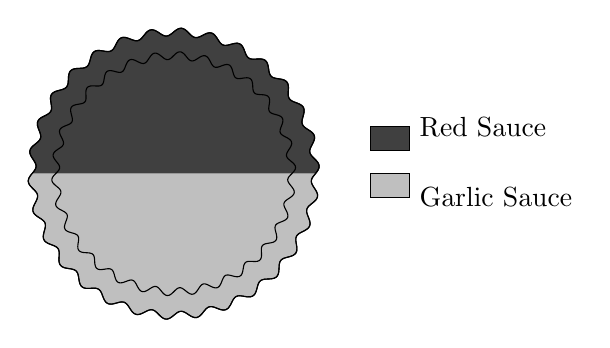
\begin{tikzpicture}
	\draw[fill=darkgray, domain=0:180,scale=1.5,samples=500] plot (\x:{1.2 + sin(\x*30)/30});
	\draw[fill=lightgray, domain=180:360,scale=1.5,samples=500] plot (\x:{1.2 + sin(\x*30)/30});
  \draw[domain=0:360,scale=1.5,samples=500] plot (\x:{1 + sin(\x*30)/30});
  \draw[domain=0:540,scale=1.5,samples=500] plot (\x:{1.2 + sin(\x*30)/30});
	
	\draw[fill=darkgray] (2.5,.3) rectangle (3,.6) node[right]  {Red Sauce};
	\draw[fill=lightgray] (2.5,0) rectangle (3,-0.3) node[right]  {Garlic Sauce};

\end{tikzpicture}
\end{center}
\caption{Pizza which is half Red Sauce and half Garlic Sauce}%
\label{fig:pizza1}%
\end{figure}
\begin{enumerate}
		\item My friend never remembers that I do not eat red sauce. Therefore, he divides the pizza so that each half has exactly half red sauce and half garlic sauce. How much is each slice of pizza worth to my friend? How much is each slice of pizza worth to me?
		%\begin{center}
	
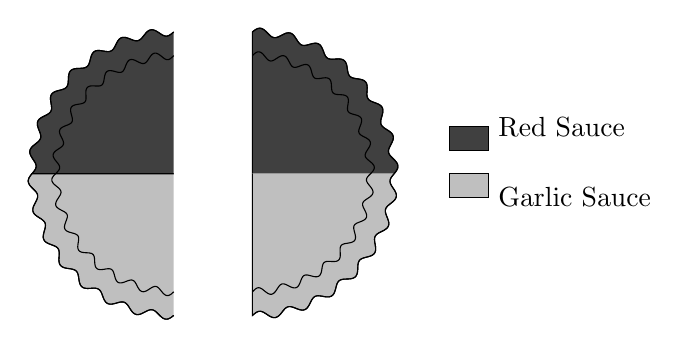
\begin{tikzpicture}[every text node part/.style={align=center}]
				\begin{scope}
						\draw[fill=darkgray, domain=90:180,scale=1.5,samples=500] plot (\x:{1.2 + sin(\x*30)/30}) -- (0,0)
	;
	\draw[fill=lightgray, domain=180:270,scale=1.5,samples=500] (0,0) -- plot (\x:{1.2 + sin(\x*30)/30})
	;
  \draw[domain=90:270,scale=1.5,samples=500] plot (\x:{1 + sin(\x*30)/30});
  \draw[domain=90:270,scale=1.5,samples=500] plot (\x:{1.2 + sin(\x*30)/30});

				\end{scope}
				\begin{scope}[xshift = 1cm]
						\draw[fill=darkgray, domain=0:90,scale=1.5,samples=500] plot (\x:{1.2 + sin(\x*30)/30}) -- (0,0)
	;
	\draw[fill=lightgray, domain=-90:0,scale=1.5,samples=500] (0,0) -- plot (\x:{1.2 + sin(\x*30)/30})
	;
  \draw[domain=-90:90,scale=1.5,samples=500] plot (\x:{1 + sin(\x*30)/30});
  \draw[domain=-90:90,scale=1.5,samples=500] plot (\x:{1.2 + sin(\x*30)/30});


	\draw[fill=darkgray] (2.5,.3) rectangle (3,.6) node[right]  {Red Sauce};
	\draw[fill=lightgray] (2.5,0) rectangle (3,-0.3) node[right]  {Garlic Sauce};

				\end{scope}

\end{tikzpicture}
%\end{center}
\fillwithlines{\stretch{1}}
	\item Suppose instead, I slice the pizza. When I do so, because I value the red sauce part as nothing, I divide the pizza so that one slice is all garlic sauce and the other slice is all red sauce. How much is each slice of pizza worth to me? How much of each slice of pizza worth to my friend? If I do the division, why is this not a fair division of the pizza? What happens if my friend is the one doing the division? Is it fair?  
	
	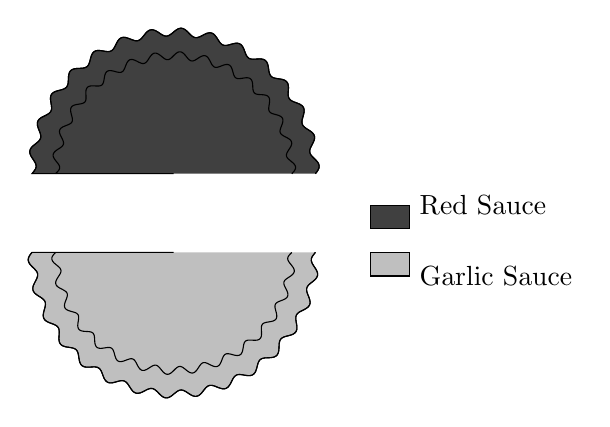
\begin{tikzpicture}[every text node part/.style={align=center}]
				\begin{scope}
						\draw[fill=darkgray, domain=0:180,scale=1.5,samples=500] plot (\x:{1.2 + sin(\x*30)/30}) -- (0,0)
	;
	%\draw[fill=lightgray, domain=180:270,scale=1.5,samples=500] (0,0) -- plot (\x:{1.2 + sin(\x*30)/30})
	%;
  \draw[domain=0:180,scale=1.5,samples=500] plot (\x:{1 + sin(\x*30)/30});
  \draw[domain=0:180,scale=1.5,samples=500] plot (\x:{1.2 + sin(\x*30)/30});

				\end{scope}
				\begin{scope}[yshift = -1cm]
						%\draw[fill=darkgray, domain=0:90,scale=1.5,samples=500] plot (\x:{1.2 + sin(\x*30)/30}) -- (0,0)
	%;
	\draw[fill=lightgray, domain=-180:0,scale=1.5,samples=500] (0,0) -- plot (\x:{1.2 + sin(\x*30)/30})
	;
  \draw[domain=-180:0,scale=1.5,samples=500] plot (\x:{1 + sin(\x*30)/30});
  \draw[domain=-180:0,scale=1.5,samples=500] plot (\x:{1.2 + sin(\x*30)/30});


	\draw[fill=darkgray] (2.5,.3) rectangle (3,.6) node[right]  {Red Sauce};
	\draw[fill=lightgray] (2.5,0) rectangle (3,-0.3) node[right]  {Garlic Sauce};

				\end{scope}

\end{tikzpicture}
\fillwithlines{\stretch{1}}
	\item Now, divide the pizza in such a way that all the red sauce is in one slice yet both slices are worth five dollars to me. How much is each slice of the pizza worth to my friend? If I do the division, why is this a fair division of the pizza? What happens if my friend is the one doing the division? Is it fair? 
	
	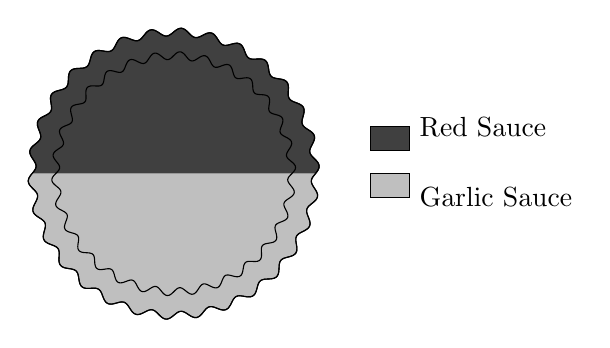
\begin{tikzpicture}
	\draw[fill=darkgray, domain=0:180,scale=1.5,samples=500] plot (\x:{1.2 + sin(\x*30)/30});
	\draw[fill=lightgray, domain=180:360,scale=1.5,samples=500] plot (\x:{1.2 + sin(\x*30)/30});
  \draw[domain=0:360,scale=1.5,samples=500] plot (\x:{1 + sin(\x*30)/30});
  \draw[domain=0:540,scale=1.5,samples=500] plot (\x:{1.2 + sin(\x*30)/30});
	
	\draw[fill=darkgray] (2.5,.3) rectangle (3,.6) node[right]  {Red Sauce};
	\draw[fill=lightgray] (2.5,0) rectangle (3,-0.3) node[right]  {Garlic Sauce};

\end{tikzpicture}
\fillwithlines{\stretch{1}}
	
\end{enumerate}

\clearpage
\subsection{Lone Divider}
%\clearpage
\studentrand
\item Three players (\randstudent[1], \randstudent[2], and \randstudent[3]) must divide cake among themselves. Suppose the cake is divided into three slices ($s_1$, $s_2$, and $s_3$). The values of the entire cake and at each of the three slices in the eyes of each of the players are shown in the following table.

\begin{center}
	\begin{tabular}{ccccc}
\hline
& Whole cake & $s_1$ & $s_2$ &$s_3$\\\hline
\randstudent[1] & \$12.00 & \$3.00 & \$5.00 & \$4.00 \\\hline
\randstudent[2] & \$15.00 & \$4.00 & \$4.50 & \$6.50 \\\hline
\randstudent[3] & \$13.50 & \$4.50 & \$4.50 & \$4.50 \\\hline 
\end{tabular}

\end{center}
 \begin{enumerate}
	\item Indicate which of the three slices are fair shares to \randstudent[1]. \fillwithlines{\stretch{1}}
	\item Indicate which of the three slices are fair shares to \randstudent[2].\fillwithlines{\stretch{1}}
	\item Indicate which of the three slices are fair shares \randstudent[3].\fillwithlines{\stretch{1}}
	\item How do you know which player divided the cake into three equal pieces?\fillwithlines{\stretch{1}}
	\item Describe a fair division of the cake.\fillwithlines{\stretch{1}}
\end{enumerate}
%\item Three players (Anna, Ben, and Cara) must divide cake among themselves. Suppose the cake is divided into three slices ($s_1$, $s_2$, and $s_3$). The values of the entire cake and at each of the three slices in the eyes of each of the players are shown in the following table.
%
%\begin{center}
	%\begin{tabular}{ccccc}
%\hline
%& Whole cake & $s_1$ & $s_2$ &$s_3$\\\hline
%Anna & \$12.00 & \$3.00 & \$5.00 & \$4.00 \\\hline
%Ben & \$15.00 & \$4.00 & \$4.50 & \$6.50 \\\hline
%Cara & \$13.50 & \$4.50 & \$4.50 & \$4.50 \\\hline 
%\end{tabular}
%
%\end{center}
 %\begin{enumerate}
	%\item Indicate which of the three slices are fair shares to Anna. \fillwithlines{\stretch{1}}
	%\item Indicate which of the three slices are fair shares to Ben.\fillwithlines{\stretch{1}}
	%\item Indicate which of the three slices are fair shares Cara.\fillwithlines{\stretch{1}}
	%\item How do you know which player divided the cake into three equal pieces?\fillwithlines{\stretch{1}}
	%\item Describe a fair division of the cake.\fillwithlines{\stretch{1}}
%\end{enumerate}
\item \boxedblank[2in]{\textbf{Lone Divider:}\ifsolns One of the players is assigned to be the divider.  The player divides the booty into equal shares (according to him).  The other players are called the choosers.  They indicate which of the shares are fair according to them.  The booty is split by giving each of the choosers one of the shares they have indicated and the divider gets the remaining share.\else \fillwithlines{\stretch{1}}\fi} 
%Make this two sections where one section is lone dider easy and the other is what to do when more than one player only bids on one plot.
\vfill \index{lone divider}

\clearpage

\item Three partners (David, Carol, and Charlotte) are dividing the plot of land among themselves using the loan divider method. Using a map, the divider (David) divides the property into three parcels $s_1$, $s_2$, and $s_3$. When the choosers bid lists are open, Carol's bid list is $\{s_1,s_2,s_3\}$ and Charlotte's bid list is $\{s_1\}$.
\begin{enumerate}
	\item Describe the fair division where David's fair share is $s_2$ \fillwithlines{\stretch{1}}
	\item Describe the fair division where David's fair share is $s_3$\fillwithlines{\stretch{1}}
\end{enumerate}


\item What should you do if both Carol and Charlotte bid $\{s_1,s_2\}$?
\fillwithlines{\stretch{1}}


\item How would you run a fair division if there were four people trying to divide an item? \fillwithlines{\stretch{2}}

\clearpage
\item We have one divider, Demon and three choosers, Chuck, Charlie, and Charles.  Demon divides the cake into four shares, $s_1, s_2, s_3$ and $s_4$.  The following table shows how each of the players values each of the four shares.  Remember that this information is private and not known to the other players.

\begin{center}
	\begin{tabular}{lcccc}
\hline
& $s_1$&$s_2$&$s_3$ & $s_4$\\\hline
Demon & 25\% & 25\% & 25\% & 25\% \\\hline
Chuck & 30\% & 20\% & 35\% & 15\% \\\hline
Charlie & 20\% & 20\% & 40\% & 20\% \\\hline
Charles & 25\% & 20\% & 20\% & 35\% \\\hline
\end{tabular}
\end{center}
\begin{enumerate}
	\item What are each player's bidding lists?
	\begin{center}
	\begin{tabular}{lp{2in}}
\hline
\ifsolns
	Demon & $s_1,s_2, s_3, s_4$\\\hline
	Chuck & $s_1, s_3$\\\hline
	Charlie &  $s_3$\\\hline
	Charles &  $s_1, s_4$\\\hline
\else
	Demon & \hspace{2in}\\\hline
	Chuck & \\\hline
	Charlie &\\\hline
	Charles &\\\hline
\fi
\end{tabular}
\end{center}
	
	\item What is the distribution
	
	Demon  \par
Chuck  \par
Charlie   \par
Charles   \par
\end{enumerate}
\fillwithlines{\stretch{1}}

\end{enumerate}

\clearpage
\HOMEWORK
%</HWHEADER>

%<*HOMEWORK>


\begin{Denumerate}
	\item \studentrand \randstudent\ buys a chocolate-strawberry-vanilla cake for \$14.00. \randPronoun\ cuts the cake into six \(60^o\) wedges as shown. \randstudent\ likes chocolate twice as much as vanilla and likes vanilla twice as much as strawberry. Calculate the value of each wedge to \randstudent. 
	
	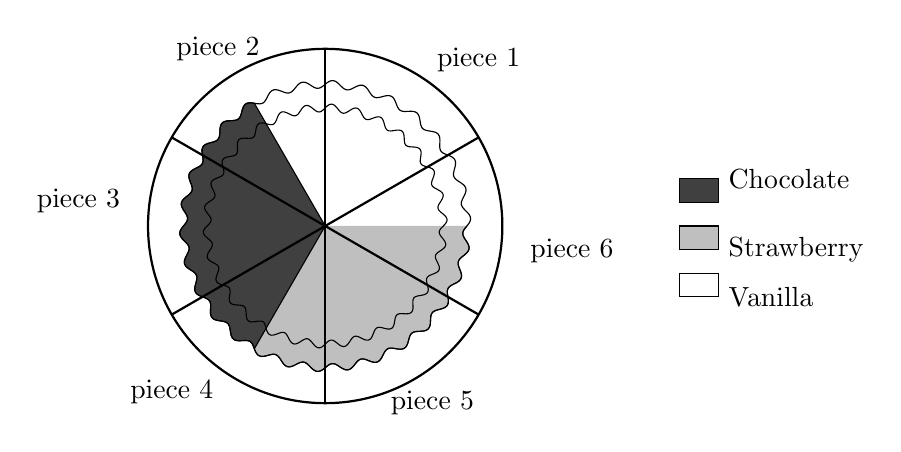
\begin{tikzpicture}
	\draw[fill=darkgray, domain=120:240,scale=1.5,samples=500] (0,0) -- plot (\x:{1.2 + sin(\x*30)/30}) 	;
	%\draw[fill=darkgray, domain=120:240,scale=1.5,samples=500] plot (\x:{1.2 + sin(\x*30)/30});
	%\draw[fill=lightgray, domain=240:360,scale=1.5,samples=500] plot (\x:{1.2 + sin(\x*30)/30});
	\draw[fill=lightgray, domain=240:360,scale=1.5,samples=500] (0,0) -- plot (\x:{1.2 + sin(\x*30)/30}) 	;
  \draw[domain=0:360,scale=1.5,samples=500] plot (\x:{1 + sin(\x*30)/30});
  \draw[domain=0:540,scale=1.5,samples=500] plot (\x:{1.2 + sin(\x*30)/30});
	
	\draw[thick,scale=1.5] (0,0) -- (30:1.5) node[above =2em] {piece 1} ;
	\draw[thick,scale=1.5] (0,0) -- (90:1.5) node[left =2em] {piece 2};
	\draw[thick,scale=1.5] (0,0) -- (150:1.5) node[below left =1.5em] {piece 3};
	\draw[thick,scale=1.5] (0,0) -- (210:1.5) node[below  =2em] {piece 4};
	\draw[thick,scale=1.5] (0,0) -- (270:1.5) node[right =2em] {piece 5};
	\draw[thick,scale=1.5] (0,0) -- (330:1.5) node[above right =1.5em] {piece 6};
	\draw[thick,scale=1.5] (0,0) circle (1.5) ;
	
\begin{scope}[xshift = 2cm]
		\draw[fill=darkgray] (2.5,.3) rectangle (3,.6) node[right]  {Chocolate};
	\draw[fill=lightgray] (2.5,0) rectangle (3,-0.3) node[right]  {Strawberry};
	\draw[] (2.5,-.6) rectangle (3,-.9) node[right]  {Vanilla};
\end{scope}

\end{tikzpicture}
\solution*{\fbox{piece 1  = \$2, piece 2 = \$3}  If you look at the whole cake, to our student, the strawberry part will be worth \$2, the vanilla part is worth \$4 and the chocolate part is worth \$8.}\vfill
	
  \item Three partners (David, Carol, and Charlotte) are dividing the plot of land among themselves using the loan divider method. Using a map, the divider (David) divides the property into three parcels $s_1$, $s_2$, and $s_3$. When the choosers bid lists are open, Carol's bid list $\{s_2,s_3\}$ and Charlotte's bid list is $\{s_1, s_3\}$.
		\begin{enumerate}
			\item Describe the fair division where David's fair share is $s_1$.
			\solution*{ \fbox{David - $s_1$, Carol - $s_2$, Charlotte - $s_3$} Because David has a fair share of $s_1$, the only other option for Charlotte is $s_3$. Since Carol will take $s_2$ or $s_3$, and $s_3$ is taken, Carol gets $s_2$.
                }\vfill
			\item Describe the fair division where David's fair share is $s_2$.
						\solution*{ \fbox{David - $s_2$, Carol - $s_3$, Charlotte - $s_1$} Because David has a fair share of $s_1$, the only other option for Charlotte is $s_3$. Since Carol will take $s_2$ or $s_3$, and $s_3$ is taken, Carol gets $s_2$.
                }\vfill
			\item Describe the fair division where David's fair share is $s_3$.
			\solution{\fbox{David - $s_3$, Carol - $s_2$, Charlotte - $s_1$}}\vfill
		\end{enumerate}
%  \begin{enumerate}
%          \item 
%                
%          \item 
%          			\solution*{
%                  \fbox{} 
%                }
%        \end{enumerate}

\hwnewpage
\studentrand
\item Four partners (\randstudent[1], \randstudent[2], \randstudent[3], and \randstudent[4]) are dividing a piece of land valued at \$480,000 among themselves using the lone-divider method. Using a map, the divider divides the property into four parcels, $s_1,s_2,s_3$ and $s_4$. The following table shows the value of each of the four parcels in the eyes of each partner, but some of the information in the table is missing.

\begin{center}
	\begin{tabular}{lcccc}
&$s_1$&$s_2 $&$ s_3$ & $s_4$\\\hline\ifsolns
\randstudent[1]  & \$80,000 & \$85,000 & \textbf{\$120,000} & \$195,000\\\hline
\randstudent[2]  & \textbf{\$125,000} & \$100,000 & \$135,000 & \$120,000\\\hline
\randstudent[3]  & \$120,000 & \textbf{\$120,000} & \$120,000 & \textbf{\$120,000}\\\hline
\randstudent[4]  & \$95,000 & \$100,000 & \textbf{\$175,000} & \$110,000 \\\hline
\else
\randstudent[1] & \$80,000 & \$85,000 & & \$195,000\\\hline
\randstudent[2] & & \$100,000 & \$135,000 & \$120,000 \\\hline
\randstudent[3] & \$120,000 & & \$120,000 &\\\hline
\randstudent[4] & \$95,000 & \$100,000 & & \$110,000 \\\hline\fi
\end{tabular}

\end{center}
\begin{enumerate}
	\item Who was the divider? Explain. \solution{\randstudent[3] because he has the same amount for every piece.}\vfill
	\item Describe the choosers' respective bid lists.
	\ifsolns
	\par
	\begin{tabular}{lcccc}
	\randstudent[1]  &  &  & $s_3$ & $s_4$\\
\randstudent[2]  & $s_1$ &  & $s_3$ & $s_4$\\
\randstudent[3]  & $s_1$ & $s_2$ & $s_3$ & $s_4$\\
\randstudent[4]  &  &  & $s_3$ & \\
	\end{tabular}\fi\vfill
	\item Described a fair division of property. \solution{\par \randstudent[1]\     $s_4$\\\randstudent[2]\  $s_1$   \\\randstudent[3]\   $s_2$  \\\randstudent[4]\    $s_3$}
	\item Explain why your answer above is the only possible fair division of the property.
	\solution{\fbox{ Basically, because \randstudent[4]\ only bids on one property, \par he starts the ball rolling.}}\vfill
\end{enumerate}
\end{Denumerate} \ENDHOMEWORK

\clearpage
%%%%%%%%%%%%%%%%%%%%%%%%%%%%%%%%%%%%%%%%%%%%%%%%%%%%%%%%%%%%%%%%%%%%%%%%%%%%%%%%%%%%%%%%%%%%%%%%%%%%%%
\subsection{Lone-Divider Case 2}

There is one complication that can happen with the lone-divider method we have not yet discussed.  It happens when two players want one and only one of the shares.  This can be solved, but requires a little more analysis.

\begin{enumerate}
	\item Dale divides the cake into three pieces $s_1$, $s_2$, and $s_3$.  The table below shows the value of the three pieces in the eyes of each of the players.
	
	\begin{center}
	\begin{tabular}{lccc}
	\hline
	 & $s_1$ & $s_2$ & $s_3$ \\\hline
	Dale & $33\frac13$\% & $33\frac13$\% & $33\frac13$\% \\\hline
	Cindy & 20\% & 30 \% & 50\% \\\hline
	Cher & 10\% & 20\% & 70\% \\\hline
\end{tabular}
\end{center}

\begin{enumerate}
	\item Describe the choosers' respective bid lists.
	\ifsolns
		Dale  $\qquad s_1,s_2, s_3$\\
	Cindy $\qquad  s_3$\\
	Cher $\qquad  s_3$\\
	\else
	\fillwithlines{\stretch{1}}
	\fi
		\item What problem do you run into when you try to divide the cake? \ifsolns \par Both Cindy and Cher only want the last piece. \else \fillwithlines{\stretch{1}}\fi
		%\vfill
%	\item Described a fair division of property.
What we are going to do is to give Dale one of the pieces that Cindy and Cher do not want, say slice $s_2$.
	\item How much are $s_1$ and $s_3$ worth together to Cindy?  to Cher? \ifsolns \par 70\% and 80\% \fi
	\fillwithlines{\stretch{1}}
	\item What you are going to to is combine $s_1$ and $s_3$ and give them to Cindy and Cher to perform a Divider-Chooser.  Explain why this will result in both Cindy and Cher receiving at least $33\frac13$\% of the cake in their eyes.  \fillwithlines{\stretch{1}}
	\item In fact, what is the minimum percentage Cindy will receive?  What is the minimum percentage Cher will receive? \ifsolns \par 35\% and 40\%\else \fillwithlines{\stretch{1}} \fi %\vfill

\end{enumerate}
%\vfill
\clearpage

	\item Three partners (David, Carol, and Charlotte) are dividing the plot of land among themselves using the loan divider method. Using a map, the divider (David) divides the property into three parcels $s_1$, $s_2$, and $s_3$. When the choosers bid lists are open, Carol's bid list $\{s_1\}$ and Charlotte's bid list is $\{s_1\}$.
\begin{enumerate}
	\item Considering that Carol only bid on the first parcel, explain how we know that parcel 2 is worth less than $1/3$ of the value of the land to Carol. Explain how we know that parcel 3 is worth less than $1/3$ of the value of the land to Carol.  \ifsolns \par \fbox{Because if they were worth at least $1/3$ of the value, they would be on the bid list.}\else \fillwithlines{\stretch{1}}\fi 
	\item Using the above information, explain how the combination of the first two parcels is worth more than $2/3$ of the value of the land to Carol. \ifsolns \par \fbox{Because what is left over is worth less than $1/3$.}\else \fillwithlines{\stretch{1}}\fi
	\item Using similar logic, explain how the combination of the first two parcels is worth more than $2/3$ of the value of the land to Charlotte.\fillwithlines{\stretch{1}}
\end{enumerate}


\end{enumerate}

\clearpage
%%%%%%%%%%%%%%%%%%%%%%%%%%%%%%%%%%%%%%%%%%%%%%%%%%%%%%%%%%%%%%%%%%%%%%%%%%%%%%%%%%%%%%%%%%%%%%%%%%%%%%
\HOMEWORK
\begin{Denumerate}

\item Six players (D,$C_1,C_2,C_3,C_4$ and $C_5$) are dividing a cake among themselves using the lone-divider method. D cuts the cake into six slices $s_1,s_2,s_3,s_4,s_5,$ and $s_6$. When the choosers' bid lists are opened, $C_1$'s bid list is $\{s_1\}$, $C_2$'s bid list is $\{s_2,s_3\}$, $C_3$'s bid list is $\{s_4,s_5\}$, $C_4$'s bid list is $\{s_4,s_5\}$, and $C_5$'s bid list is $\{s_1\}$. Describe how to proceed to obtain a fair division of the cake.
\solution{ There are  many correct solutions.  They all include $C_2$ getting either $s_2$ or $s_3$.  
$C_3$ and $C_4$ getting either $s_4$ or $s_5$ and the other one going to the other, and $C_1$ and $C_5$
splitting the combination of $s_1$ and another piece which are then split using divider-chooser.}
\vfill
\fillwithlines{\stretch{1}}
\item We have one divider, Demon and three choosers, Chuck, Charlie, and Charles.  Demon divides the cake into four shares, $s_1, s_2, s_3$ and $s_4$.  The following table shows how each of the players values each of the four shares.  Remember that this information is private and not known to the other players.

\begin{multicols}{2}
\begin{center}
	\begin{tabular}{lcccc}
\hline
& $s_1$&$s_2$&$s_3$ & $s_4$\\\hline
Demon & 25\% & 25\% & 25\% & 25\% \\\hline
Chuck & 15\% & 20\% & 50\% & 15\% \\\hline
Charlie & 20\% & 20\% & 40\% & 20\% \\\hline
Charles & 25\% & 20\% & 20\% & 35\% \\\hline
\end{tabular}
\end{center}
\begin{enumerate}
	\item What are each player's bidding lists?
	
	\begin{center}
	\ifsolns
	\begin{tabular}{lcccc}
	Demon  &  $s_1$ & $s_2$ & $s_3$  &  $s_4$\\
Chuck  &  &  & $s_3$  & \\
Charlie  &  &  & $s_3$  & \\
Charles  &  $s_1$ &  &  &  $s_4$ \\
	\end{tabular}
	\else
	\begin{tabular}{lp{2in}}
\hline
%& $s_1$&$s_2$&$s_3$ & $s_4$\\\hline
Demon & \\\hline
Chuck & \\\hline
Charlie &  \\\hline
Charles &  \\\hline
\end{tabular}\fi
\end{center}
\end{enumerate}
	\end{multicols}
	\begin{enumerate}
	
  \setcounter{enumi}{2}
	\item How are you going to make a fair division?
	\solution{Similar to the previous problem, Charles gets	 $s_1$ or	 $s_4$, Demon gets something, and Chuck and Charlie will take the combination of $s_3$ and another slice and perform divider-chooser.}
	
\fillwithlines{\stretch{1}}
\end{enumerate}




\end{Denumerate} \ENDHOMEWORK
%%%%%%%%%%%%%%%%%%%%%%%%%%%%%%%%%%%%%%%%%%%%%%%%%%%%%%%%%%%%%%%%%%%%%%%%%%%%%%%%%%%%%%%%%%%%%%%%%%
%\clearpage
%\subsection{Lone Chooser}
%
%The lone chooser method was proposed in 1964 by A.M. Fink, a mathematician at Iowa State University and a Wartburg College graduate.  The lone chooser method is an iterative process that generalizes to multiple players more easily than the lone divider method. 
%
%\begin{enumerate}
%	\item \vfill
%	\item \vfill
%	\item \vfill
%
%\end{enumerate}
%
%\clearpage

\clearpage
\subsection{Method of Sealed Bids} 
\index{sealed bids} \studentrand
Sometimes you want to split up items without physically cutting them apart.  For example, suppose \randstudent[1]\ is living with two roommates and everyone is graduating.  Over the years, they have purchased some appliances together and now they need to fairly divide the appliances.  

In the method of sealed bids, each roommate is going to write down what they believe is a fair value for each appliance and seal the ``bids'' in an envelope.  When the envelopes are opened, we get the following results:

\begin{tabular}{llll}
 &  \randstudent[1]  &  \randstudent[2]  &  \randstudent[3] \\\hline
 T.V.  &  \$75  &  \$100  &  \$120 \\\hline
 Microwave  &  \$35  &  \$30  &  \$40 \\\hline
 Crock Pot  &  \$5  &  \$10  &  \$7 \\\hline
 Toaster Oven  &  \$7  &  \$10  &  \$5 \\\hline
 Blender  &  \$20  &  \$25 &  \$20 \\\hline\ifsolns
 Total &\$142	&\$175	&\$192 \\\hline
Fair Share &\$ 47.33	&\$	58.33&\$ 64.00\\\hline
 \else
 Total &\$	&\$	&\$ \\\hline
Fair Share &\$	&\$	&\$ \\\hline
 \fi
 
\end{tabular}
\begin{enumerate}
	\item How much does each person think the whole property to be split is worth?  What would be their fair share? 
	\ifsolns  \$47.33 	 \$58.33 	 \$64.00 
\else
	\fillwithlines{\stretch{1}}
\fi
	
	\item How would you propose splitting up the property?
\fillwithlines{\stretch{1}}
	%\vfill
	
	\clearpage
	
	\item Method of Sealed Bids
	\begin{enumerate}
	\item Assign each item to the highest bidder.  Who gets what?
	\begin{center}
	\large
	\begin{tabular}{lp{3in}}
	Roommate & Items  \\\hline \ifsolns
	Rachel & \\\hline
	 Sally &   Crock Pot, 
 Toaster Oven, 
 Blender 
\\\hline
	 Theresa & T.V., 
 Microwave 
\\\hline
\else
		\randstudent[1] & \\\hline
	 \randstudent[2] &  \\\hline
	 \randstudent[3] &\\\hline
\fi
	\end{tabular}
\end{center}
\normalsize
	\item What is the total value of the items to the winners?  Use the prices they have assigned themselves.
	\begin{center}
	\large
		\begin{tabular}{lcccc}
	Roommate & Value  & Fair Share & Cash Paid & Cash Received\\\hline
\ifsolns
Rachel  &  &  \$47.33  &    &  \$47.33 \\\hline
 Sally  &  \$45.00  &  \$58.33  &    &  \$13.33 \\\hline
 Theresa  &  \$160.00  &  \$64.00  &  \$96.00  &    \\\hline
\else
	\randstudent[1] & \$ \\\hline
	 \randstudent[2] & \$ \\\hline
	 \randstudent[3] & \$ \\\hline
	\fi
	\end{tabular}
\normalsize
\end{center}	 
	 \item Which of the roommates have received more than their fair share of the property?  How much more did they receive? \label{sb1}

	 \item Which of the roommates have received less than their fair share of the property?  How much less did they receive? \label{sb2}
	\item Have the roommates who received too much pay cash for the extra value of the property over and above their fair share.  Pay the roommates who did not receive enough the shortfall between what they see as a fair share and the value of the property they have received.
	\item How much cash do you have left? \solution{ \$35.33} 
	\item Divide the extra cash by 3 and give each roommate one third of the extra cash.
	\ifsolns
	\begin{tabular}{lcr}
Roommate  & \\
\randstudent[1]  &  \$59.11 \\
 \randstudent[2]  &  \$25.11  & Crock Pot,  Toaster Oven,  Blender\\
 \randstudent[3]  &  \$(84.22) & T.V.,  Microwave\\
\end{tabular} \else
	\fillwithlines{\stretch{1}}
\fi
	

\item Explain how each roommate has received a fair share.
	\fillwithlines{\stretch{1}}
	

\item What are some of the drawbacks of the  method of sealed bids?

\fillwithlines{\stretch{1}}
\end{enumerate}


\clearpage

\item Five heirs ($A,B,C, D,$ and $E$) are dividing an estate consisting of six items using the method of sealed bids.  The heirs bids on each of the times are given in the following table.

\begin{center}
	\begin{tabular}{c c c c c c}
	& $A$ & $B$ & $C$ & $D$ & $E$ \\\hline
	\ifsolns
	Item 1  &  \$352.00  &  \$295.00  &  \$395.00  &  \$368.00  &  \$324.00 \\\hline
Item 2  &  \$98.00  &  \$102.00  &  \$98.00  &  \$95.00  &  \$105.00 \\\hline
Item 3  &  \$460.00  &  \$449.00  &  \$510.00  &  \$501.00  &  \$476.00 \\\hline
Item 4  &  \$852.00  &  \$825.00  &  \$832.00  &  \$817.00  &  \$843.00 \\\hline
Item 5  &  \$513.00  &  \$501.00  &  \$505.00  &  \$505.00  &  \$491.00 \\\hline
Item 6  &  \$725.00  &  \$738.00  &  \$750.00  &  \$744.00  &  \$761.00 \\\hline\hline
Total &  \$3,000.00  &  \$2,910.00  &  \$3,090.00  &  \$3,030.00  &  \$3,000.00\\\hline
\else
Item 1 & \$352 & \$295 & \$395 & \$368 & \$324 \\\hline
Item 2 & \$98 & \$102 & \$98 & \$95 & \$105 \\\hline
Item 3 & \$460 & \$449 & \$510 & \$501 & \$476 \\\hline
Item 4 & \$852 & \$825 & \$832 & \$817 & \$843 \\\hline
Item 5 & \$513 & \$501 & \$505 & \$505 & \$491 \\\hline
Item 6 & \$725 & \$738 & \$750 & \$744 & \$761 \\\hline\hline
Total &  &  &  &  & \\\hline
Fair Share &  &  &  &  & \\\hline \fi

\end{tabular}

\end{center}
\begin{enumerate}
	\item Describe the first settlement of this estate and compute the surplus cash. 
	\ifsolns
	\$130 
	
	\begin{tabular}{lrccc}
 & Items & Fair Share & Initial Cash & Final Cash\\\hline
$A$   &  4,5  &   \$600.00   &   \$(765.00)  & (\$739.00)	\\\hline
 $B$   &    &   \$582.00   &   \$582.00   & \$608.00 	\\\hline
 $C$   &  1,3  &   \$618.00   &   \$(287.00)  & (\$261.00)	\\\hline
 $D$   &    &   \$606.00   &   \$606.00   & \$632.00 	\\\hline
 $E$  &  2,6  &   \$600.00   &   \$(266.00)  & (\$240.00)	\\\hline
\end{tabular} \else
	\fillwithlines{\stretch{1}}
\fi
	

	\item Describe the final settlement of this estate.
	\fillwithlines{\stretch{1}}
	

\end{enumerate}

\end{enumerate}

\clearpage
%%%%%%%%%%%%%%%%%%%%%%%%%%%%%%%%%%%%%%%%%%%%%%%%%%%%%%%%%%%%%%%%%%%%%%%%%%%%%%%%%%%%%%%%%%%%%%%%%%%
\HOMEWORK
%</HWHEADER>

%<*HOMEWORK>


\begin{Denumerate}
  \item Aden, Ben, and Charles are dividing four pieces of furniture using the method of sealed bids.  Their bids on each of the items are given in the following table.
  
\begin{center}
	  \begin{tabular}{cccc}
 & Aden & Ben & Charles \\\hline
 Dresser & \$150 & \$300 & \$275 \\\hline
 
 Desk & \$180 & \$150 & \$165 \\\hline
 
 TV Cabinet & \$170 & \$200 & \$260 \\\hline
 Tapestry & \$400 & \$250 & \$500 \\\hline \hline
\ifsolns 
Total & \$900 & \$ 900 & \$1200\\\hline
Fair Share & \$300 & \$300 & \$400\\\hline
\else
Total &  &  & \\\hline
Fair Share &  &  & \\\hline
\fi
\end{tabular}

\end{center}
		\begin{enumerate}
			\item Describe the first settlement of the items and compute the Surplus.
			\solution*{ Aden gets the Desk and \$120, Ben gets the Dresser, Charles gets the TV Cabinet and the Tapestry, but pays in \$360.  There is a surplus of \$240.
                }\vfill
			\item Describe the final settlement of the items.\vfill
				\solution*{ Aden gets the Desk and \$200, Ben gets the Dresser and \$80, Charles gets the TV Cabinet and the Tapestry, but pays \$280.
                }\vfill
			\end{enumerate}
	\item Kathy, Susie, and Judy are equal partners in a small bookstore.  They can't get along anymore, but they don't want to  sell the bookstore to an outsider so they decide to settle the matter using the method of sealed bids. Kathy bids \$240,000 for the business, Susie bids \$210,000, and Judy bids \$225,000.  Describe the final settlement of this bookstore.
			\solution{As the highest bidder, Kathy receives the store and owes \$155,000, Susie receives \$ 75,000  and Judy receives \$ 80,000. 
			}\vfill
\hwnewpage
		\item Three women (Carrie, Jeri, and Violet) share an apartment and wish to divide the chores: bathrooms, cooking, dishes, laundry, and vacuuming.  For each chore, they privately write the least they are willing to receive monthly (their negative valuation) in return for doing that chore.  The results are shown in the following table.
		
		\begin{center}
	\begin{tabular}{lccc}
 & Carrie & Jeri & Violet \\\hline
 Clean bathrooms & \$-20 & \$-30 & \$-40 \\\hline
 Do cooking & \$-50 & \$-10 & \$-25 \\\hline
 Wash dishes & \$-30 & \$-20 & \$-15 \\\hline
 Mow the lawn & \$-30 & \$-20 & \$-10 \\\hline
 Vacuum and dust & \$-20 & \$-40 & \$-15 \\\hline 
\end{tabular}
\end{center}
Divide the chores using the method of sealed bids.  Who does which chores?  Who gets paid, and how much? Who pays, and how much? 
		\solution*{Carrie cleans the bathrooms and pays \$12.  Jeri does the cooking and pays \$12.  Violet washes the dishes, mows the lawn, vacuums and dusts and gets paid \$23 (or \$24 with rounding).
		}

\end{Denumerate} \ENDHOMEWORK
%%%%%%%%%%%%%%%%%%%%%%%%%%%%%%%%%%%%%%%%%%%%%%%%%%%%%%%%%%%%%%%%%%%%%%%%%%%%%%%%%%%%%%%%%%%%%%%%%%%%%
\clearpage 
%\solnstrue
\clearpage
\section{Study Guide}


To prepare for the exam over this chapter,
you should review the in-class worksheets and homework.
Be ready to do the kind of problems you faced on the homework.

As a general guide, I recommend reviewing the following topics.

\begin{enumerate}
  \item Know what it means for a division of assets to be fair.
  \item Calculate the fair division by method of
        \begin{enumerate}
          \item Divider-Chooser
          \item Lone-Divider
          \item Sealed Bids
        \end{enumerate}
  \item Know what to do when two players want one and only one piece of the division.
  \item Apportionment
        \begin{enumerate}
          \item Know how to find the Standard Divisor and the Standard Quota.
          \item Understand the quota rule.
   				\item Be able to understand when a modification of the apportionment problem violates the Population Paradox.
   				\item Be able to understand when a modification of the apportionment problem violates the New States Paradox.
   				\item Be able to understand when a modification of the apportionment problem violates the Alabama Paradox.
        \end{enumerate}
   \item Given an apportionment problem, be able to find the apportionment using Hamilton's Method.
    \item Given an apportionment problem, be able to find the apportionment using Jefferson's Method.
    \item Given an apportionment problem, be able to find the apportionment using Adam's Method.
    \item Given an apportionment problem, be able to find the apportionment using Webster's Method
\end{enumerate}

%</WORKSHEETS>

\endinput
